\subsection{Computational Complexity}
Computational complexity is the study of the time and space resources required to solve computational problems. The task of computational complexity is to prove lower bounds on the resources required by the best possible algorithm for solving a problem, even if that algorithm is not explicitly known.\\
The chief distinction made in computational complexity is between problems which can be solved using resources which are bounded by a polynomial in n, or which require resources which grow faster than any polynomial in n. In the latter case we usually say that the resources required are {\it exponential} in the problem size.\\
The 'polynomial increase' mentioned in {\it Strong Church-Turing Thesis} is this polynomial class only. So, the strong Church Turing Thesis says that any algorithm which can be run on some mode of computation can be run on the probabilistic Turing machine in p(k) where k is number of elementary operations required in that mode of computation and p({$\cdotp$}) is a polynomial function.\\
By {\it Strong Church-Turing Thesis}, we can say that if an algorithm can not be run( in polynomial time) on the probabilistic Turing machine,then it can't be run on any machine. Thus, the strong Church–Turing thesis implies that the entire theory of computational complexity will take on an elegant, model-independent form if the notion of efficiency is identified with polynomial resource algorithms, and this elegance has provided a strong impetus towards acceptance of the identification of 'solvable with polynomial resources'  and  'efficiently solvable'.

\subsection{Complexity Classes}
A {\bf Complexity Class} contains a set of problems that take a similar range of space and time to solve, for example "all problems solvable in polynomial time with respect to input size," "all problems solvable with exponential space with respect to input size," and so on. Some complexity classes may be a subset of others. The following figure shows various complexity classes along with there relation(Some relations are not yet proved. E.g.: it is still unknown whether NP = P on not).
\begin{figure}[h!]	
	\centering
	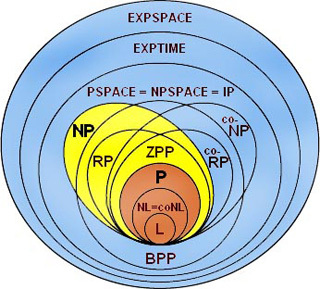
\includegraphics{images/Complexity.jpg}\par
	\caption{Various Complexity Classes}
	\label{fig:complexity}
\end{figure} 

\subsubsection{P Class}
The class P contains decision problems (problems with a \enquote{yes} or \enquote{no} answer) that are solvable in polynomial time by a deterministic Turing machine. A problem in P can be solved in $n^k$ time for some constant k and where n is the size of the input.\\ 
Some famous problems in P include:
\begin{itemize}
\item Finding if the given numbers are relatively prime(and in general prime too)
\item Linear Programming
\item Greatest Common Divisor
\end{itemize}

\subsubsection{NP and co-NP Class}
The class NP contains decision problems (problems with a \enquote{yes} or \enquote{no} answer) that are solvable by a Turing machine in non-deterministic polynomial time — this includes problems that are solvable in polynomial time up to problems that are solvable in exponential time. While they can take a long time to solve, problems in NP can be verified by a Turing machine in polynomial time. This means that if given a yes answer to an NP problem, you can check that it is right in polynomial time. This yes answer is often called a witness or a certificate.\\
More rigorously, a language L is in NP if there is a Turing machine M with the following properties:
\begin{enumerate}
\item If x $\in$ L then there exists a witness string w such that M halts in the state $q_Y$ (yes state) after a time polynomial in size of x when the machine is started in the state x-blank-w.
\item If x $\in$ L then for all strings w which attempt to play the role of a witness, the
machine halts in state $q_N$(no state) after a time polynomial in size of x when M is started in the state x-blank-w.
\end{enumerate}
Language of an algorithm/problem can be understood as the set of all the inputs which results in the \enquote{yes} state.\\
If a problem X is in NP, then its complement, $\overline{X}$ is in coNP. coNP contains problems that have a polynomial time verification for \enquote{no} answers — if given a solution that does not solve the problem, it is easy to verify if that solution does not work.\\\\
{\bf Relations between P, NP and coNP}\\
\[ P \subseteq NP \]
\[ P \subseteq coNP \]
hence, \[ P=NP \cap coNP \]
It is still unknown whether {$P = NP$}. In such a case {$ P=NP=coNP $}. If {$ P \neq NP $}, it will lead to a new class, {\bf NPI } (NP intermediate) which are not solvable in polynomial time but can be verified in polynomial time. \\
An important class of problems in {\it NP} class is the {\it NP-complete}.

\subsubsection{NP-Complete Problems}
 {\it NP-complete } problems are very special because any problem in the {\it NP} class can be transformed or reduced into {\it NP-complete} problems in polynomial time. This means that if you can solve an {\it NP-complete} problem, you can solve any other problem in {\it NP}. An important consequence of this is that if you could solve an {\it NP-complete} problem in polynomial time, then you could solve any {\it NP} problem in polynomial time. \\
The famous \href{https://en.wikipedia.org/wiki/Cook-Levin_theorem}
{\bf Cook-Levin Theorem} establishes the {\it NP-Completeness} of {\scshape CSAT}.
\\\\ \href{https://en.wikipedia.org/wiki/Boolean_satisfiability_problem}
{\scshape CSAT: }Given a Boolean circuit composed of {\scshape and,or} and {\scshape not} gates, is there an assignment of values to the inputs to the circuit that results in the circuit outputting 1,that is, is the circuit satisfiable for some input?\\
All the other problems are shown to be {\it NP-Complete} by reducing {\scshape CSAT} or previously determined {\it NP-Complete} problem to that problem and using the {\it transitivity} of {\it reduction}.\\
Some famous {\it NP-Complete} problems are:
\begin{itemize}
\item Knapsack problem
\item Graph isomorphism
\item Hamiltonian Path Problem
\end{itemize} 

\subsubsection{PSPACE Class}
The class PSPACE is the set of decision problems that can be solved by a deterministic Turing machine in a polynomial amount of space with respect to the input size. \\\\
{\bf Relations between P, NP and PSPACE:}
\[ P \subseteq PSPACE \]
\[ NP \subseteq PSPACE \]
\[ PSPACE \subseteq EXP \]
The final relation including the P,NP, PSAPCE, L({\it Logarithmic Space}) and EXP({\it Exponential Time}) is:
\[ L \subseteq P \subseteq NP \subseteq PSPACE \subseteq EXP \]
It is known that {$P \not\equiv EXP$} and {$L \not\equiv PSPACE$}. So, at least one of the inclusions is strict.

